\begin{document}

\chapter{Results}

Unfortunately, diachronic embeddings, which is trained for the purpose of tracing the change of word representations in vector space models, are met with challenges in how the training is evaluated. In this study, the trained embeddings are first examined in interactive interface in order to explore the structure of the diachronic embeddings. Furthermore, analogical reasoning and bootstrapping methods are employed as an attempt to pinpoint the properties of embeddings that might be influenced by the source data.

\section{Evaluation on analogical reasoning}

The training of word embeddings are evaluated based on intrinsic and extrinsic evaluations.  

Analogical thinking and context-dependent evidence lay a cognitive ground for the studies of semantic change (Traugott, 2017). In terms of vector space models, analogical thinking is associated with the directionality of vectors that represent words in pairs or in groups. Despite its popularity, wide application, and the much effort into the expansion of datasets, the analogical reasoning task is not adaptable for diachronic or historical word embeddings \parencite{wevers2020digital}. In our pilot study, the CA8 dataset, established by Li et al. (2018), is adopted to explore semantic relations in the trained embeddings. The dataset 8 does not rely heavily on geographical locations and proper nouns as the target. Instead, 8 relational types are included; in particular, among the 1,307 analogical word pairs in the type of “nature,” 282 of them are single-character word pairs, and the semantic relations are rich and elemental, including “number, time, animal, plant, body, physics, weather, reverse, color” (Li et al., 2018). By solving the 3COSADD and 3COSMUL objectives (Levy and Goldberg, 2014), we found that 26 and 35 word pairs are successfully identified across all time periods within small and large window sizes. For example, pairs like 東-西:左-右 ‘east-west:left-right’, 真-假:左-右 ‘realfake: left-right’, and 冷-熱:南-北 ‘cold-hot:south-north’, are solved in all time periods, and the pair 冰-水:雪-雨 ‘ice-water:snow-rain’ is also stably analogous except in 1980s. Based on the preliminary findings, we will continue the extraction and analysis of analogous pairs. Firstly, we will develop a list of word pairs derived from existing datasets (e.g., Google testset, BATS testset), dictionaries, thesauri, and the Chinese WordNet sense inventory. Then, the list will be used for the pair-based methods. The coverage of solved pairs indicates the inverted degrees of semantic change in analogous pairs. Below are the preliminary results of solved coverages on our trained diachronic character embeddings.

\section{Stability of \textsc{BOOTSTRAP} diachronic embeddings}

\begin{figure}[H]
  \centering
  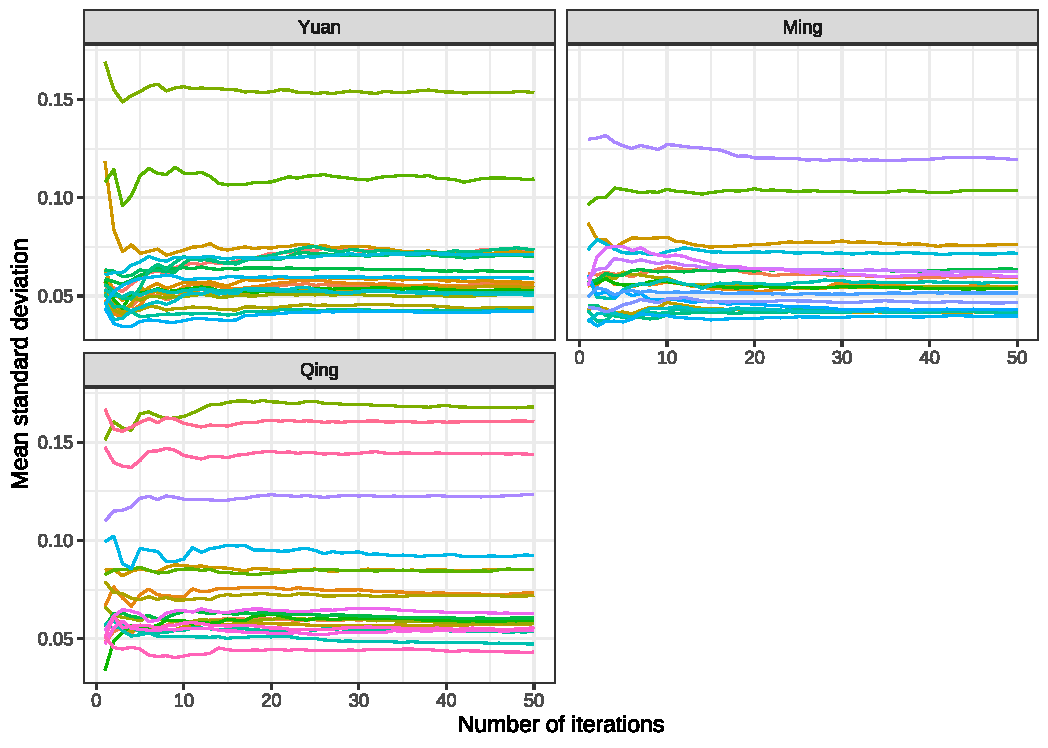
\includegraphics[width=0.95\textwidth,keepaspectratio]{figures/stability_plot_mean_std}
  \caption{Stability over iterations based on query words extracted from LDA topic models and 20 nearest neighbors from \textsc{fixed} embeddings}
  \end{figure}

\section{Collocational-based approach}
The results of the VNC periodization are plotted as dendrograms (See \fref{fig:all_VNC}, \fref{fig:pre_VNC}, and \fref{fig:post_VNC}%, and the vector tables of collograms are provided in Appendix \ref{appendix:all_jia}, \ref{appendix:pre_jia}, and \ref{appendix:post_jia}.

\begin{figure}[H]
\centering
\begin{minipage}[b]{0.3\linewidth}
  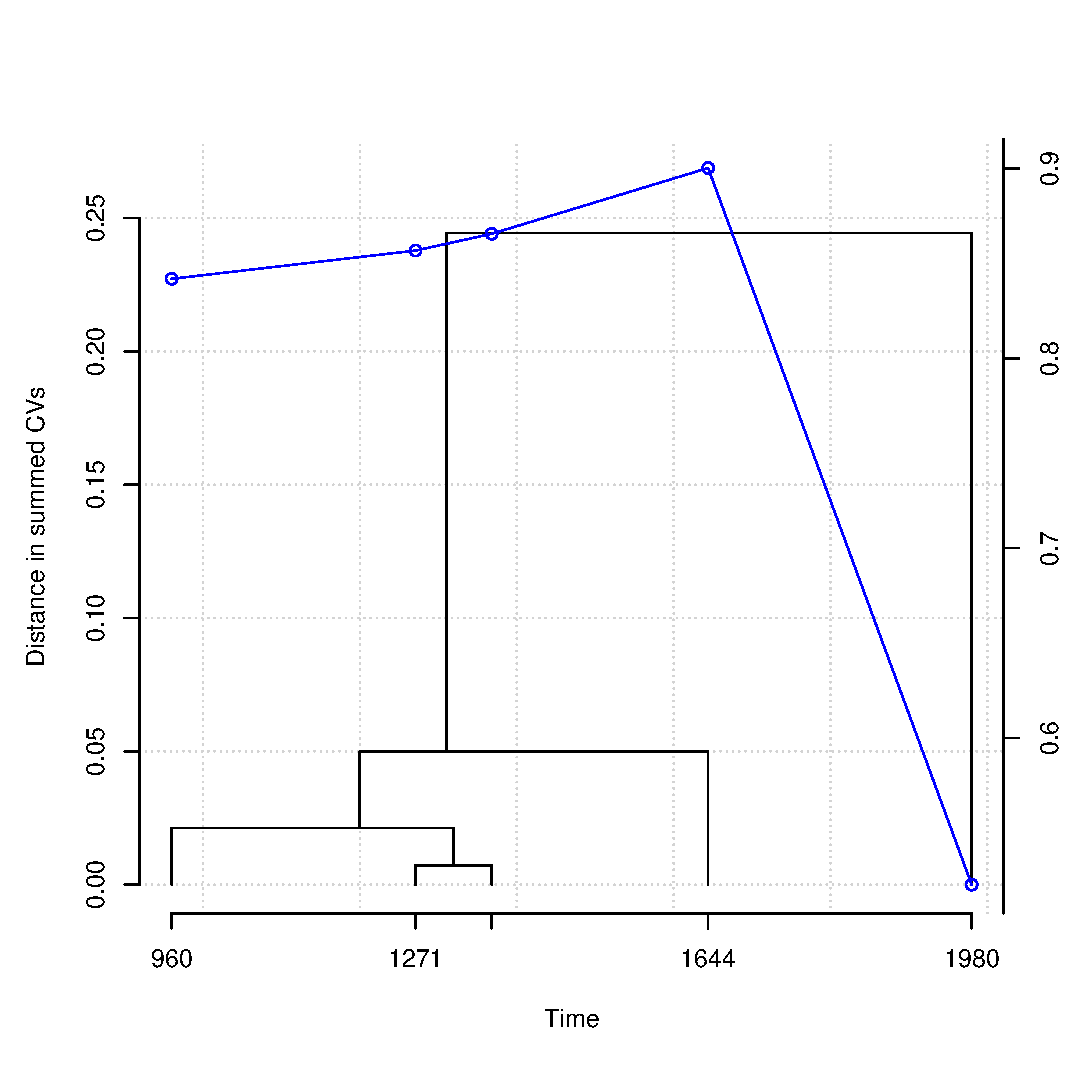
\includegraphics[width=\textwidth]{figures/pre_VNC_cor.eps}
  \caption{VNC periodization of collograms occuring before \jia}
  \label{fig:pre_VNC}
\end{minipage}
\quad
\begin{minipage}[b]{0.3\linewidth}
  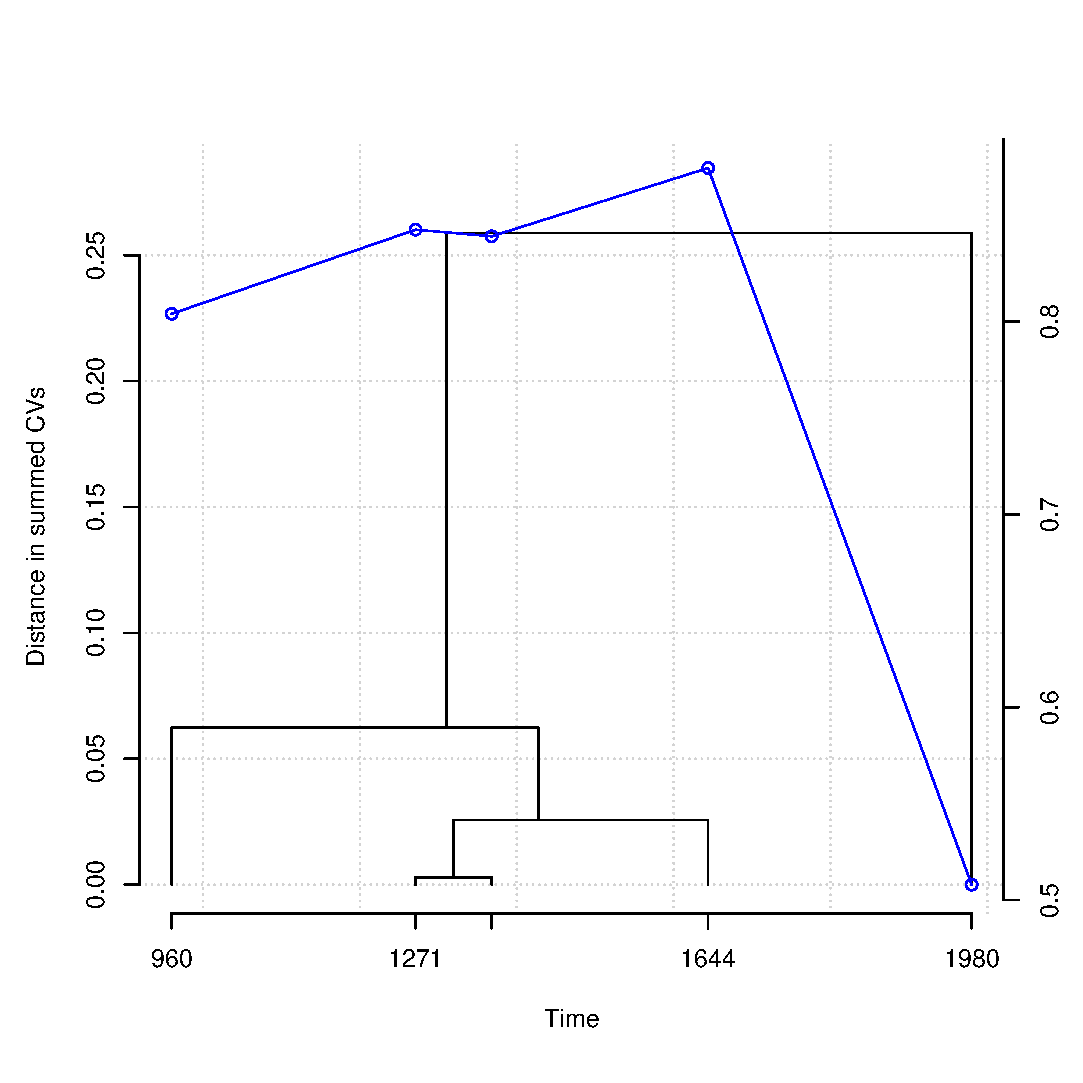
\includegraphics[width=\textwidth]{figures/post_VNC_cor.eps}
  \caption{VNC periodization of collograms occuring after \jia}
  \label{fig:post_VNC}
\end{minipage}
\quad
\begin{minipage}[b]{0.3\linewidth}
  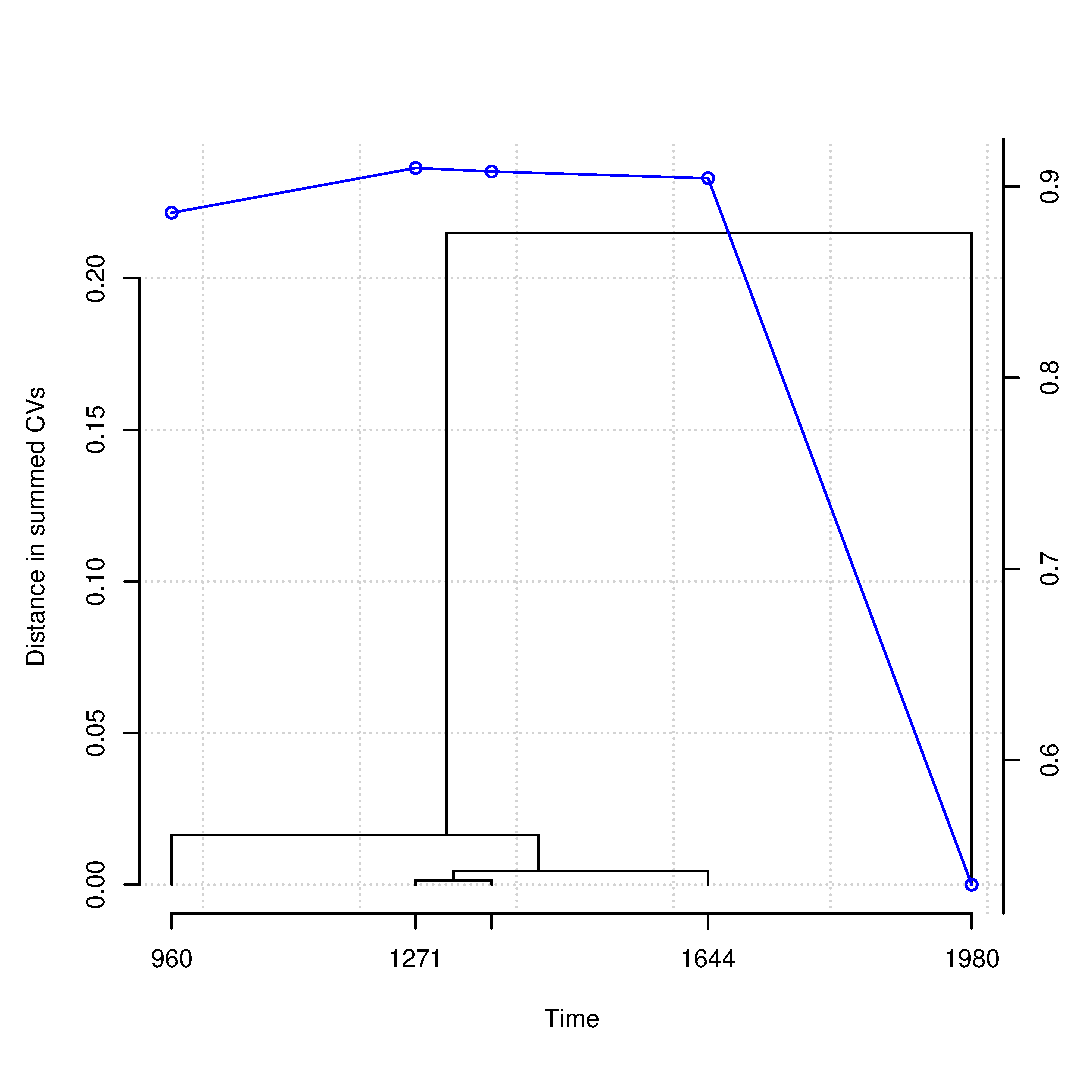
\includegraphics[width=\textwidth]{figures/all_VNC_cor.eps}
  \caption{VNC periodization of collograms occuring with \jia}
  \label{fig:all_VNC}
\end{minipage}
\end{figure}

The correlation between the Qing dynasty and 1980s shows a drastically decreasing trend compared to that of its predecessor, the Ming dynasty and the Qing dynasty, marking a distinct new stage of development. Furthermore, the flattening of the line at 2 clusters in the scree plot suggests no subgroups are identified. It is generalized from the results of the \gls{vnc} method that while modern Chinese is drastically different from pre-modern Chinese, the timeframe from the Tang dynasty to the Qing dynasty shows that each dynasty is dissimilar from one another and cannot be merged, even for the shortest dynasty Yuan. The granularity of diachronic data is not equally partitioned.

% \begin{exe}
%   \ex (Tang)\\魏賈,\CJKfakebold{家累}千金,博學善著作。--段成式《酉陽雜俎》卷七·酒食 \parencite{sturgeon2019ctext}
%   \ex (Tang)\\不使鄉人治驛路, 卻將\CJKfakebold{家累}宿山雲。--姚合 送河中楊少府宴崔駙馬宅
%   \ex (Song)\\\CJKfakebold{家傳}筆法學光堯,聖草真行說兩朝。--楊皇后 宮詞·其二十八
%   \ex (Ming)\\\CJKfakebold{家語}云:與好人同行,如霧露中行,雖不濕衣,時時滋潤。
%   \ex (Ming)\\\CJKfakebold{國家}既遷河朔--漕船志 席書
%   \ex (Ming)\\習侈難反故\CJKfakebold{世家}之能保者寡矣--恥言 徐禎稷
% \end{exe}

\section{Diachronic word embeddings}
\begin{figure}[H]
\centering
\begin{minipage}[b]{0.45\linewidth}
  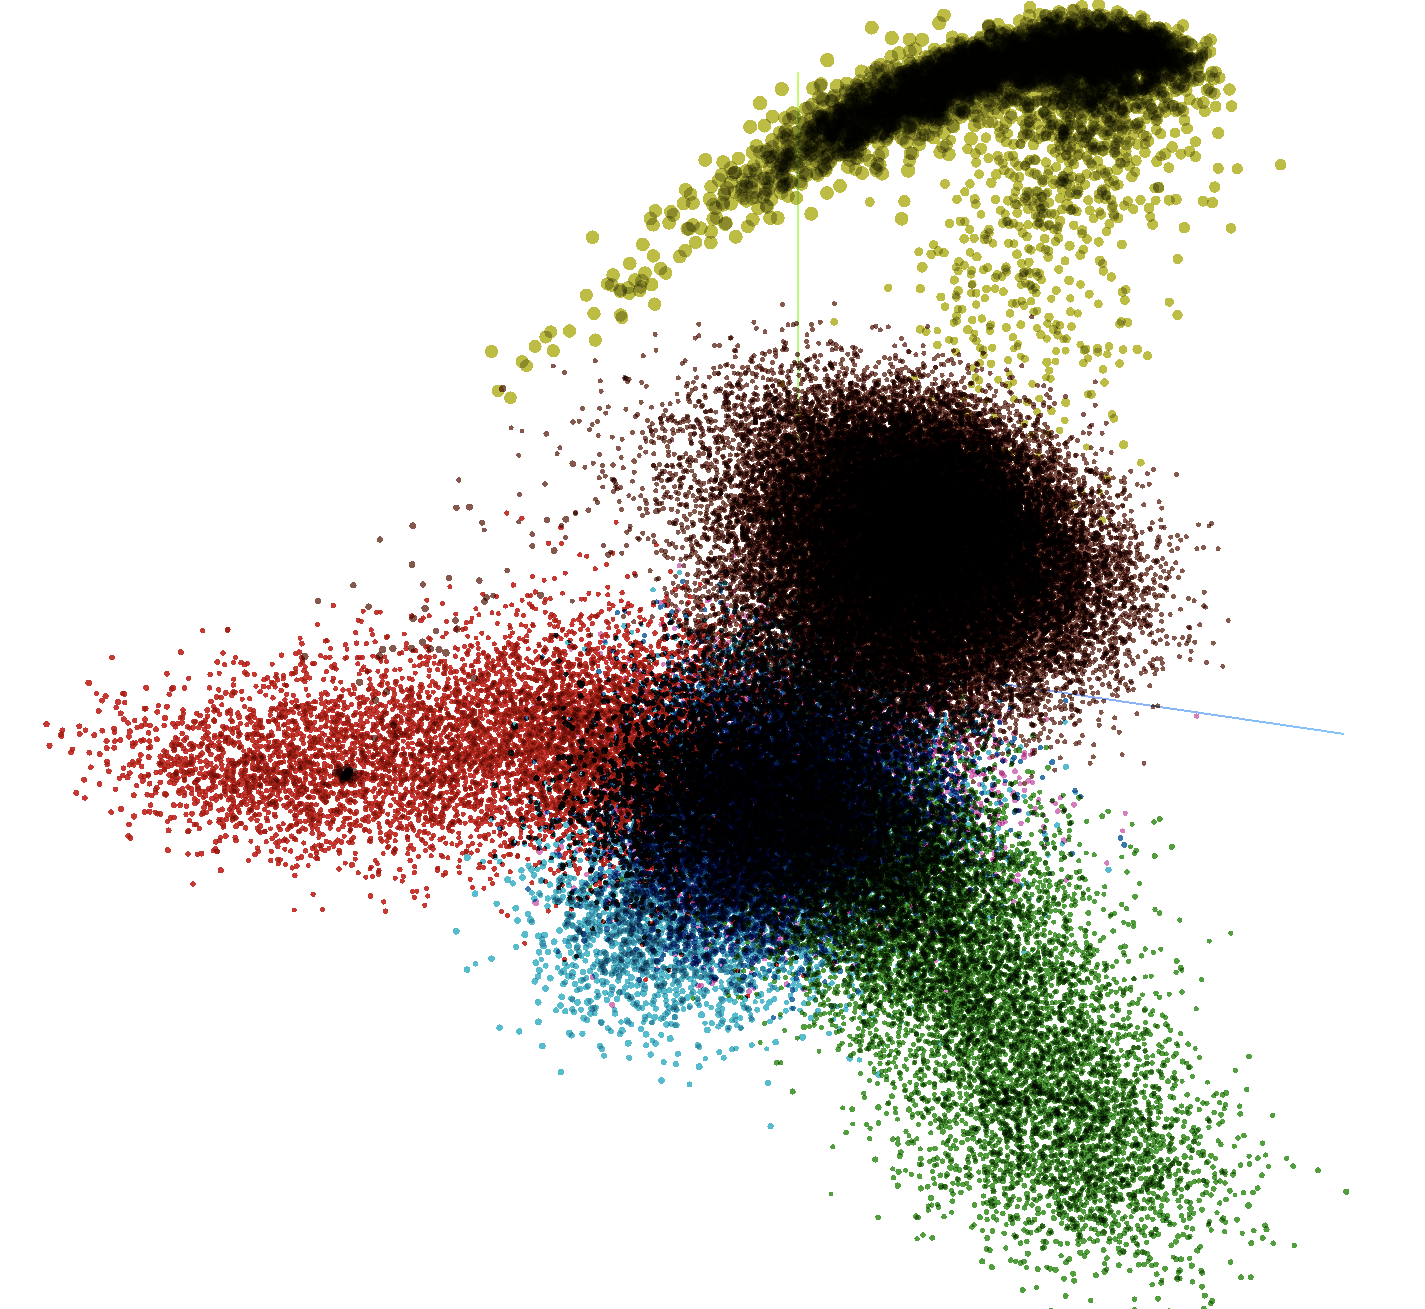
\includegraphics[width=\textwidth]{figures/pca_embedding_projector}
\end{minipage}
\quad
\begin{minipage}[b]{0.45\linewidth}
  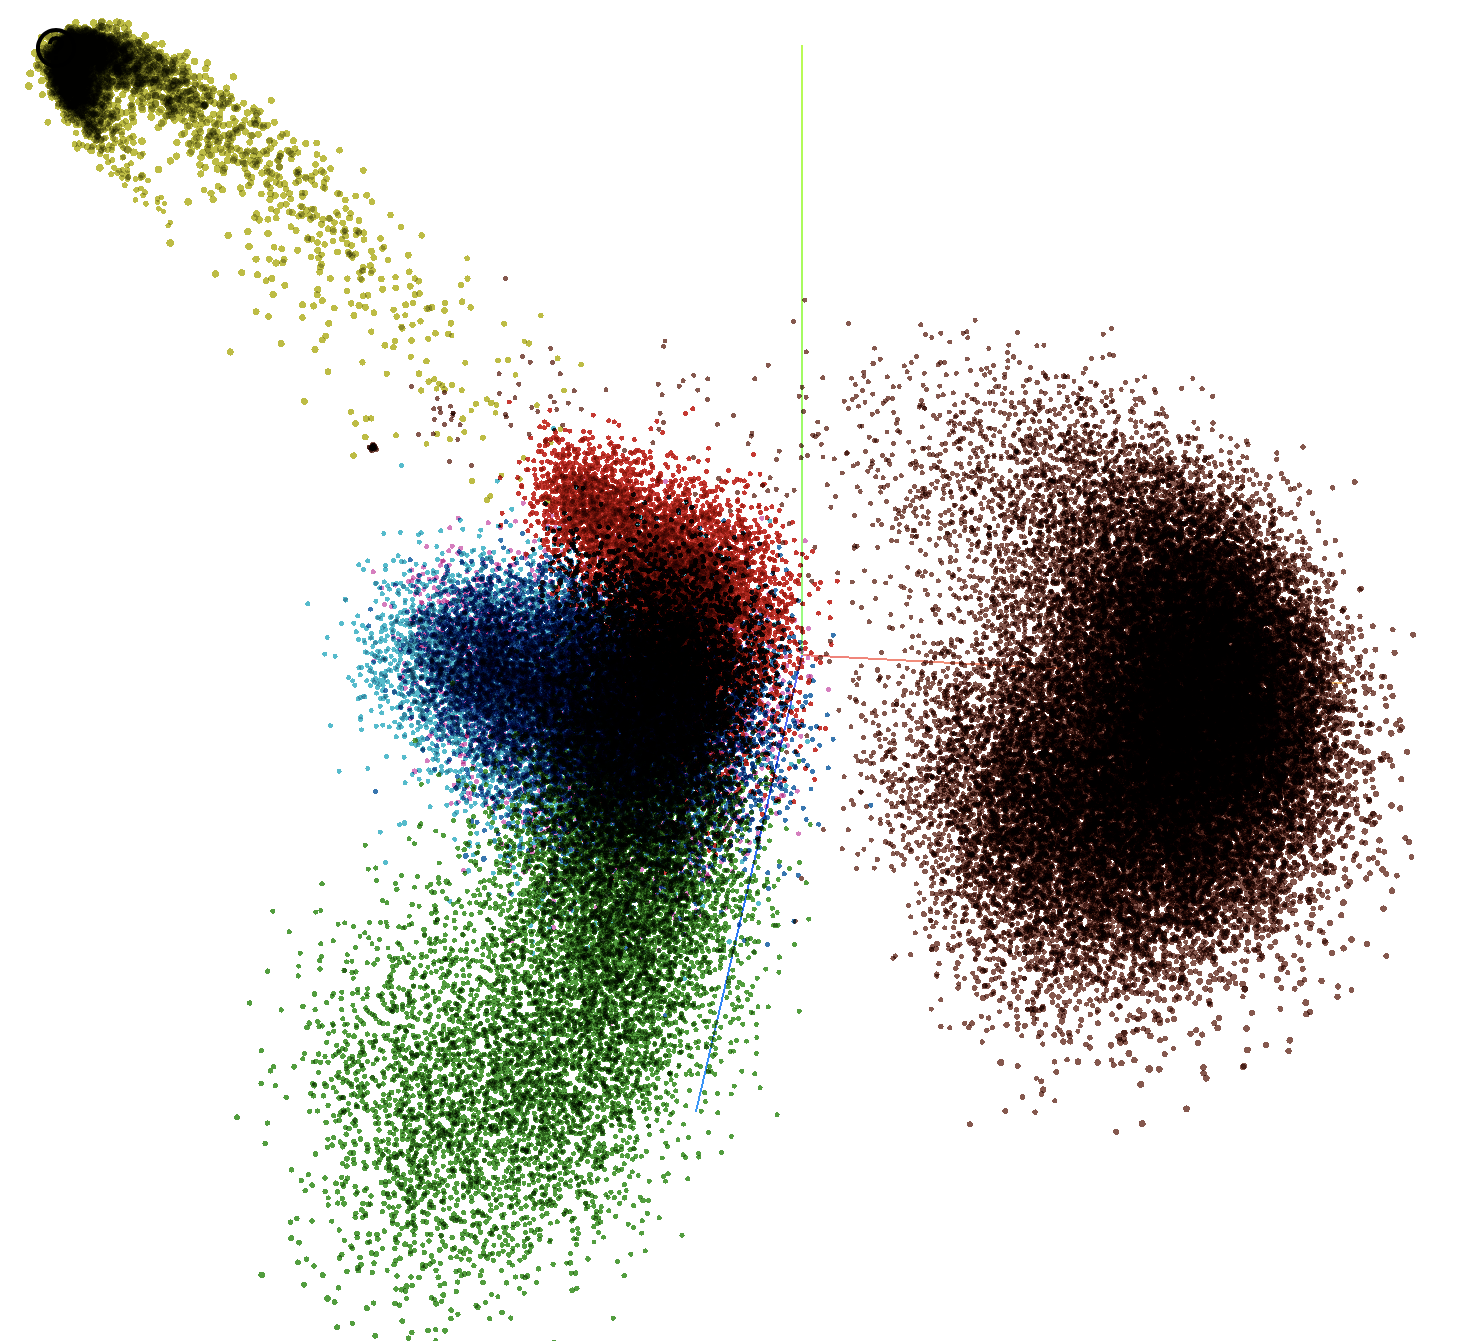
\includegraphics[width=\textwidth]{figures/pca_embedding_projector_2}
\end{minipage}
\caption{Snapshot of PCA Embedding Projector in TensorBoard\\\footnotesize{* Total variance described: 34.6\%.\\* Tang (dark blue); Song (red); Yuan (pink); Ming (sky blue); Qing (green); 1980s (brown); 2010s (mustard).}}
\end{figure}

\begin{figure}[H]
\centering \begin{minipage}[b]{0.45\linewidth}
  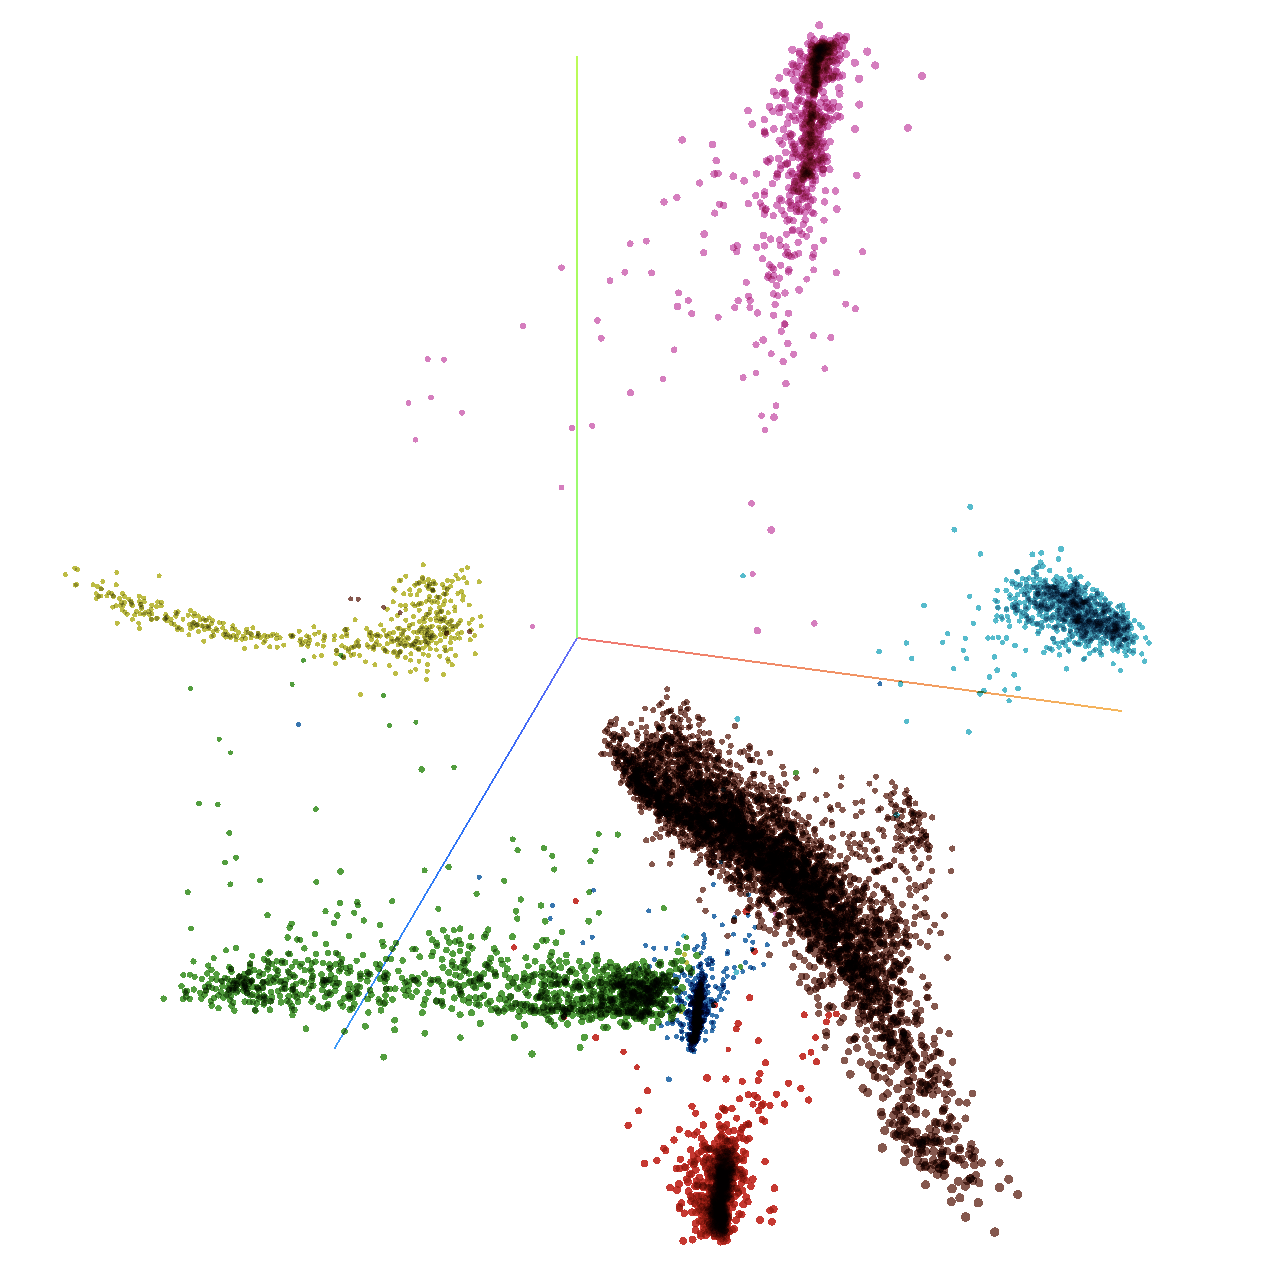
\includegraphics[width=\textwidth]{figures/tsne_embedding_projector_67}
\end{minipage}
\quad \begin{minipage}[b]{0.45\linewidth}
  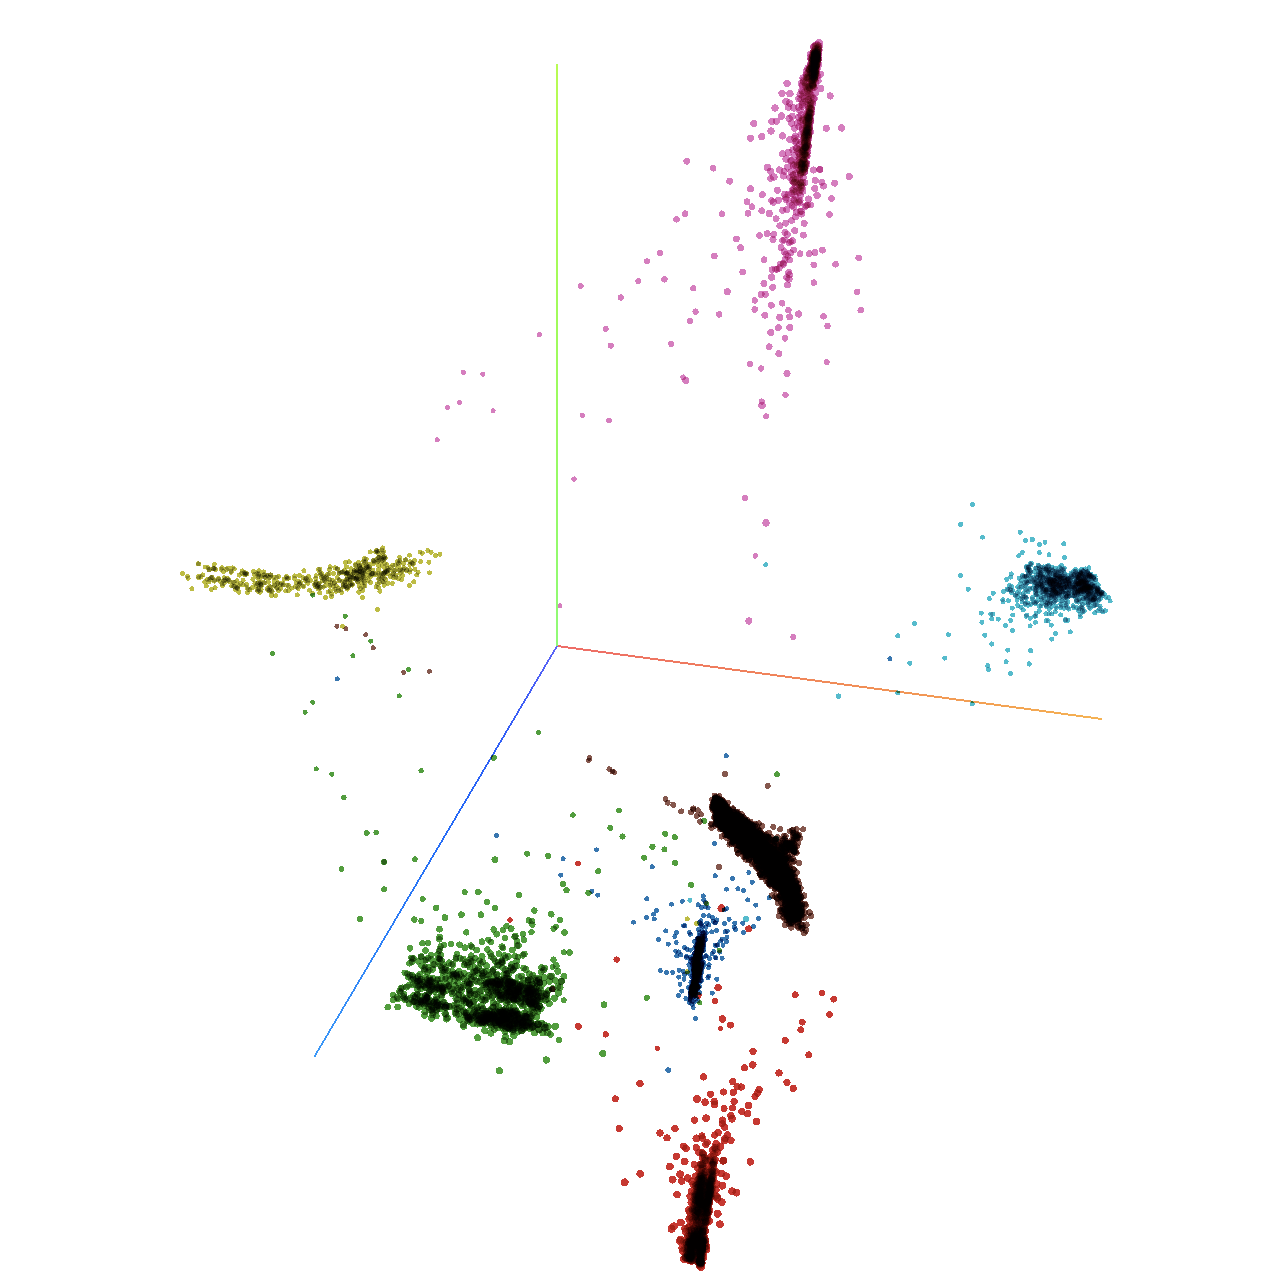
\includegraphics[width=\textwidth]{figures/tsne_embedding_projector_102}
\end{minipage}
\caption{Snapshot of t-SNE Embedding Projector in TensorBoard\\\footnotesize{* Perplexity: 74; learning rate: 10\\Iteration: 67 (left panel); 102 (right panel)\\* Tang (dark blue); Song (red); Yuan (pink); Ming (sky blue); Qing (green); 1980s (brown); 2010s (mustard).}}
\end{figure}

After word embeddings from Tang dynasty to Qing dynasty are generated, 10 words with the highest cosine similarity scores of jia are extracted from each dynasty. Character-based results are shown in Fig. 1, and word-segmented results are provided in the Appendix. It is found that character-based word embeddings yield a set of words with meanings that are closer to the definitions listed in the OED and MOE dictionaries.

Nonetheless, it is probable that zhong `burial mound' tops the list because it could be coded for its resemblance of strokes to jia, or because the word was also used to refer to the eldest male offspring in the family, as in jia-zhong and zhong-fu `wife of the eldest male offspring.' From the perspective of nearest neighboring words \parencite{hamilton2016cultural}, the core meanings of jia remains stable from pre-modern time, indicating a strong association with the family clan and the role of a wife, as in zu and qi. Secondly, the words li `village; neighborhood' and cun `village; country' are evident of the structured social unit of living from pre-modern time. However, the nearest neighboring words of li falls into the category of measurement units such as zhang `one-tenth of chi' and chi, whereas zun is still closely linked to words like zhuang `village; town' and xiang `lane; valley.' Interestingly, the most semantically related words to jia in pre-modern Chinese time depicts the idea of home more as a social concept than a physical one. If such words as zhi `nephew', zi `offspring', and sao `sister-in-law' are considered, it becomes clearer that word vectors are able to capture the cultural aspect of jia in pre-modern Chinese. 
Noticeably, on the list of most similar words are two words related to money—fu `to be wealthy' and zi `to estimate (value).' Although they do not appear as frequently as the aforementioned words, they are assigned higher similarity scores than shi `era; decades' and guo `nation; feudal land', which are thought of as one aspect of core meanings of jia, as in guo-jia `nation; state.'

\begin{figure}[H]
\centering
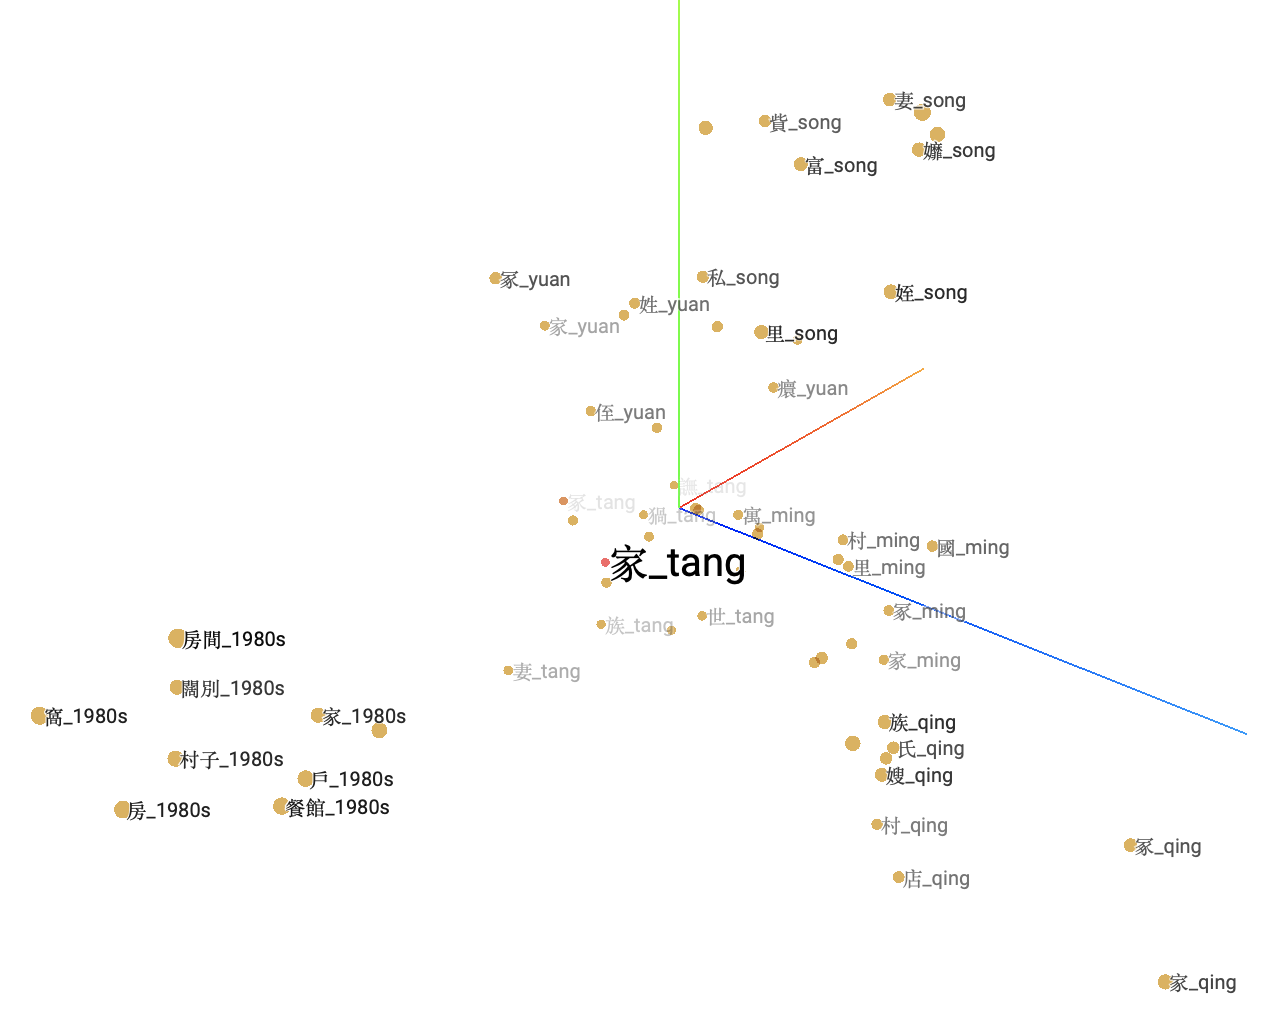
\includegraphics[height=0.45\textheight,width=0.85\textwidth,keepaspectratio]{figures/jia_neighboring_words}
\caption{Neighboring words of \jia projected in a three-dimensional space}
\label{fig:jia_neighboring_words}
\end{figure}

\begin{table}[H]
    \centering
    \begin{tabular}{@{}c@{\hspace{1ex}}l@{\hspace{0.5ex}}l@{\hspace{0.5ex}}l@{\hspace{0.5ex}}l@{\hspace{0.5ex}}l@{\hspace{0.5ex}}l@{\hspace{0.5ex}}l@{\hspace{0.5ex}}l@{\hspace{0.5ex}}l@{\hspace{0.5ex}}l@{\hspace{0.5ex}}l@{}}
    \toprule
      \multicolumn{1}{c}{Time} &
      \multicolumn{1}{c}{Word} &
      \multicolumn{10}{c}{Nearest neighboring words} \\
    \midrule
      Tang & 家 & 冢, &族, &冡, &妻, &猧, &世, &富, &譕, &教, &國\\
      Song & 家 & 冢, &族, &里, &富, &貲, &妻, &姪, &私, &貴, &孊\\
      Yuan & 家 & 冢, &族, &貲, &妻, &睮, &姓, &世, &侄, &癏, &侲\\
      Ming & 家 & 冢, &族, &妻, &豕, &里, &村, &寓, &富, &國, &產\\
      Qing & 家 & 冢, &村, &族, &氏, &妻, &店, &子, &寓, &病, &嫂\\
    \cmidrule{1-12}
      \multirow{4}{*}{1980s} &
    %   \multicolumn{1}{c}{\multirow{2}{*}{1980s}} &
        家 & 房間, &村子, &闊別, &戶, &家小, &酒店, &窩, &房, &旗下, &餐館 \\
      & 家庭 & 婚姻, &小家庭, &職業婦女, &家族, &單親, &兩性, &同儕, &貧苦, &上班族, &鄰里 \\
      & 家人 & 親友, &親人, &部屬, &親朋好友, &同事, &師長, &親戚, &父母親, &妻兒, &異性 \\
      & 家族 & 豪門, &母系, &氏族, &超人氣, &白種, &救星, &文化人, &族, &小家庭, &宗派 \\
    \cmidrule{1-12}
      2010s &
      家 & 離開, &感受, &要求, &安慰, &遇見, &聽到, &身上, &早上, &傷害, &陪伴\\
    \bottomrule
    \end{tabular}
    \caption{Neighboring words with the highest similarity scores to the words \jia, \zh{家庭}{jiātíng}{family/household}, \zh{家人}{jiārén}{family members}, \zh{家族}{jiāzú}{a family's clan}.}
    \label{tab:my_label}
\end{table}

\gls{asbc} and Dcard are representative of the concept of jia in the late 20\textsuperscript{th} and 21\textsuperscript{st} century. As Table 2 shows, cun-zi `village' are still closely related to the concept of jia, appearing as one of its semantically most similar words in the vectors of both window size 1 and 5. Furthermore, more words carrying the meaning of family are seen on the list of \gls{asbc}, including jia-xiao `wife and children', quan-jia `the whole family', and yi-jia `(a) family', yet zu and qi are no longer seen, which might reflect the shift of family clans as units of living to smaller household sizes and more equal status of each family member. 

Secondly, not the word yu `apartment', but hu `one-paneled door; household', wo `nest; hiding place', and fang `house; room' are used to refer to jia as a physical space or unit of living. Because of the emergence of these alternative words, home evolves to be a private sphere \parencite{mallett2004understanding}. These words highlight the physical aspect of meaning of jia and its characteristics under transformation. The word wo can be used either as a noun or a verb, and as a verb, it stresses that home is portrayed as a place where we feel cozy and at ease, and where we can ``retreat and relax'' \parencite{mallett2004understanding}. 

Interestingly, aside from wo as a verb, kuo-bie `to be separated for a long time' is the only verb on the list of \gls{asbc}, and the concept of home as a ``journeying'' experience recurs in the Dcard corpus, as in li-kai `to leave' \parencite{mallett2004understanding,samanani2019house}. Besides, terms of commercial properties are spurring in the list of most similar words to jia, including jiu-dian `hotel', can-quan `restaurant; bistro', lu-quan `hotel', xiao-chi dian `eatery.' It is speculated that commercialization is accountable for this new trend, but it is also possible that jia starts to be used as a classifier, as in yi-jia-lu-quan `one hotel.' Judging from the data in \gls{asbc}, it is seen that not only does the concept of jia changes across time, but the word use of jia changes as well, which is evident in more alternative word choices to refer to the concept of jia. 

In the 21\textsuperscript{st} century, the word jia is associated with a wider variety of words, mostly verbs. Unlike data from earlier time spans, the words are less semantically associated with the direct naming of a physical space or family unit, but because people engage themselves more an d more often in describing their daily life and encounters, verbs like li-kai `to leave', qan shou `to-feel', shang-hai `to hurt', and pei-ban `to accompany' are assigned the highest probabilities to words of jia. 

Although word embedding technique grows increasingly prevalent in the field of computational linguistics and natural language processing, it has been criticized for representing words with multiple meanings as one single vector, which is referred to as ``meaning conflation deficiency'' \parencite{camacho2018survey} To allow the algorithms to know different senses of the same word form, two main methods for sense embeddings are proposed. [21, 22] One is unsupervised as senses are ``induced'' from the training corpora; the other is knowledge-based, meaning external sense inventories, such as WordNet, are required to fine-tune the word vector models. 

Since the keyword jia does not reveal how people are connected in this recent era, 2 other keywords are chosen to see if more insights can be gained. The words jia-ren and jia-ting can help us understand the social structure of home nowadays. As the above figure shows, the concept of jia is first depicted with a single word jia, and as time passes, jia is conceptualized with multiple other lexical items. In other words, in earlier time, different aspects of home are described by the character jia, yet these aspects are embodied with different words such as jia ren-ren and jia-ting in modern Chinese texts.

% to-do
% 從 semantic displacement (Hamilton, 2016) 的結果來看,前幾名的字易受「詞頻」、「連綿詞」的影響,因此可先篩選「中頻詞」、「非連綿詞」,重新看排名。

\begin{figure}[H]
\centering
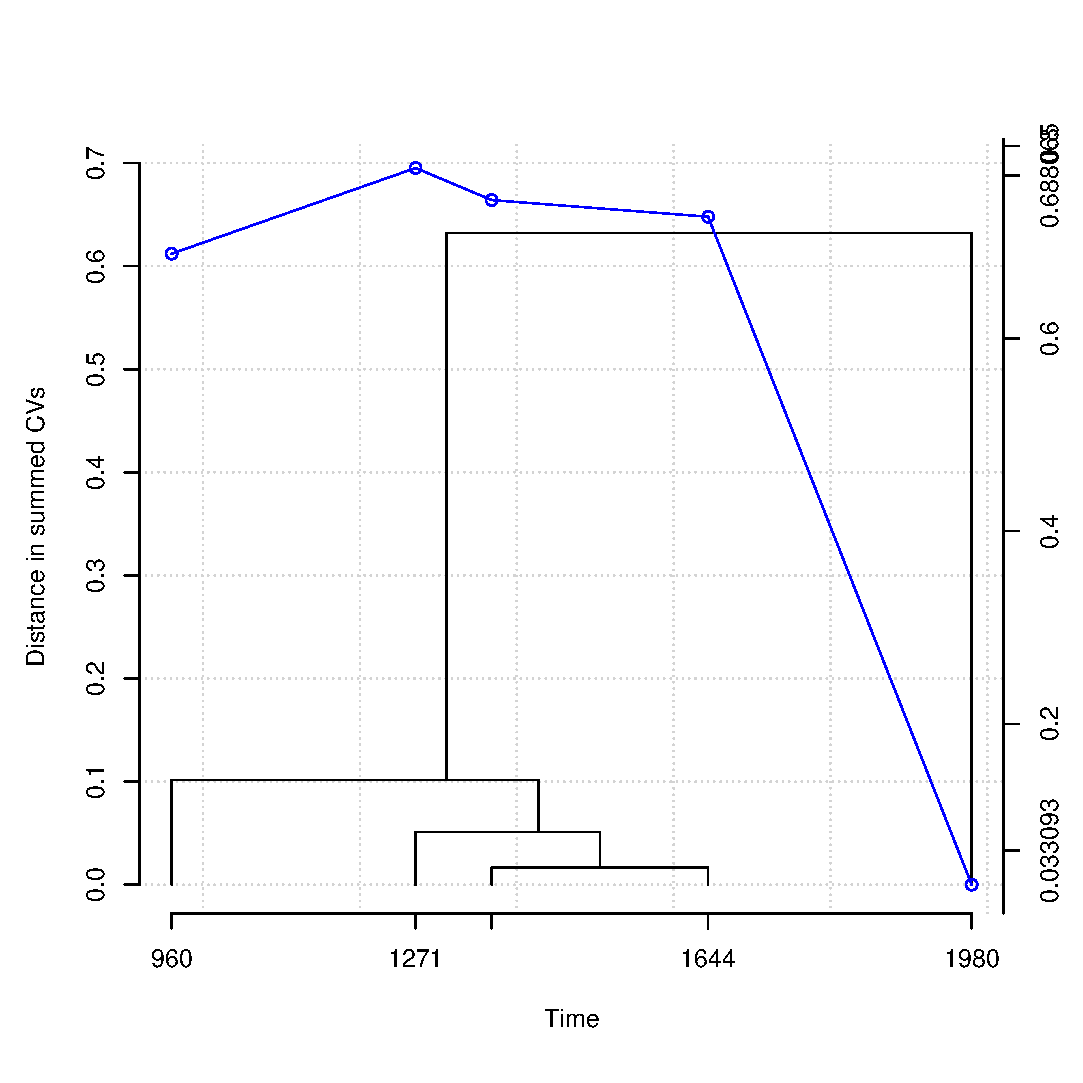
\includegraphics[height=0.45\textheight,width=0.45\textwidth,keepaspectratio]{figures/sim_cor.eps}
\caption{VNC results of word-level embeddings}
\label{fig:sim_VNC}
\end{figure}

% \section{morphology}
% \noindent Criteria are set to include more lexical items.
% 並列語詞
% 偏正語詞
% 聯綿詞(是不可分析的偶字詞,主要是雙聲疊韻詞)
% 複音詞(包括加詞綴或疊字之語詞,類似派生詞)
% 專名
% 其他結構(不在以上諸類的)might include 音譯詞、述賓\parencite{wei1997corpus,chang2008,wang2005jia,沈孟穎2015台灣現代住宅設計之轉化}

\section{Diachronic sense embeddings}
\begin{figure}[H]
    \centering
    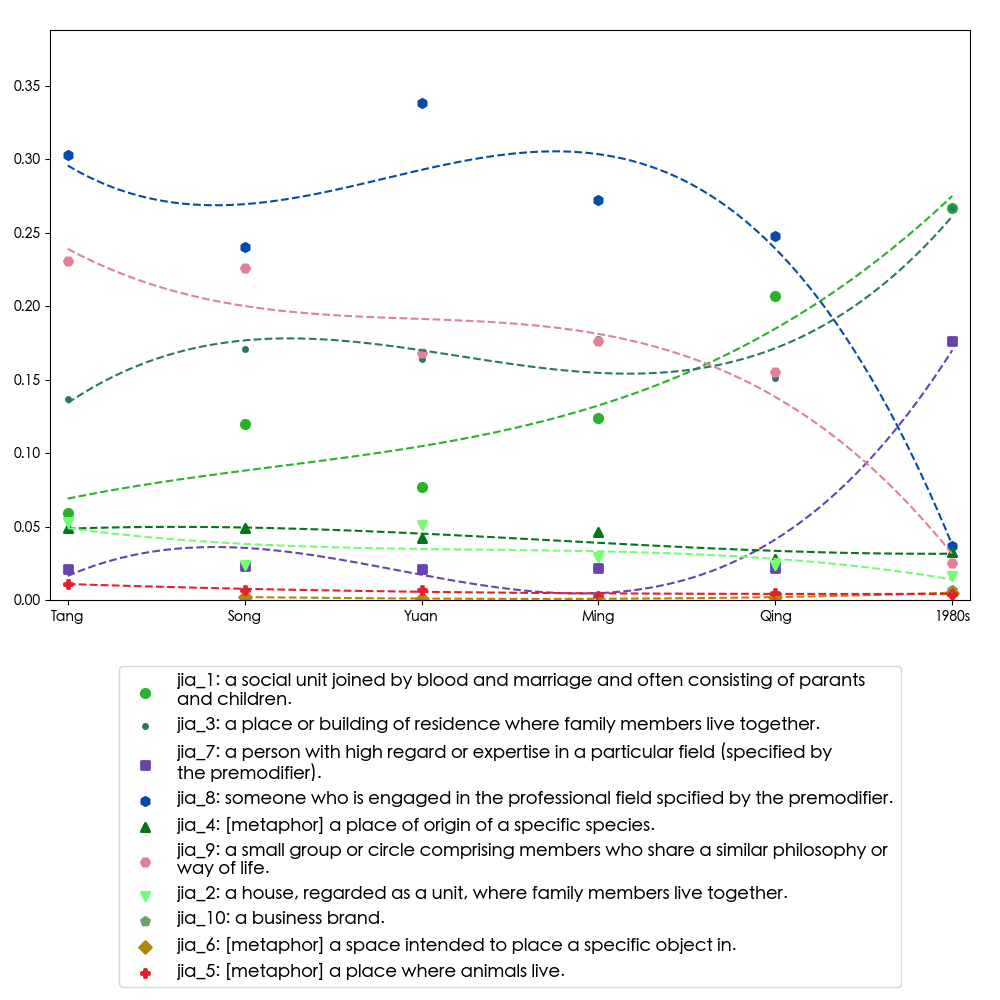
\includegraphics[width=0.85\textwidth]{figures/jia_en}
    \caption{Diachronic interactions of senses}
    \label{fig:jia_en}
\end{figure}

% \begin{exe}
%   \ex
% (Sense 7)\\
% 又以堪輿\CJKfakebold{家}所謂龍脈也 \parencite{sturgeon2019ctext}\\
% yòu\_\_yǐ\_\_kānyújiā\_\_suǒwèi\_\_lóngmài\_\_yě\\
% additionally\_\_P\_\_geomantician\_\_so-called\_\_dragon's-vein\_\_PAR\\
% \textit{what[=the terrain] a geomantician would call a dragon's vein}
% \end{exe}

The polysemy of a lexical item is addressed by constructing multiple contextualized token embeddings. Shades of meanings are reflected in the diversity of contextual use.

The results indicate that \jia enjoy far global distance but low local distance, and suddenly rises during 1980s.

\end{document}